\documentclass[11pt]{article}
\begin{figure}[t]
\usepackage{tikz}
\usetikzlibrary{arrows.meta,calc,decorations.markings,decorations.pathmorphing}

% Styling helpers
\tikzset{
    axisline/.style={very thick, black},
    corecircle/.style={thick, dashed, gray},
    knotline/.style={ultra thick, blue!65},
    swirlarrow/.style={-{Stealth[length=3mm,width=2mm]}, thick},
    vline/.style={-{Stealth[length=3mm,width=2mm]}, thick, teal!70!black},
    tube/.style={line width=6pt, line cap=round},
    ghost/.style={opacity=0.25},
    labelbox/.style={fill=white, inner sep=2pt, rounded corners=2pt},
}

\usetikzlibrary{knots,hobby,calc,intersections,decorations.pathreplacing,shapes.geometric,spath3}
\centering
\begin{tikzpicture}[scale=0.9]

% === parameters ===
\def\R{3.0} % torus major radius
\def\r{1.0} % torus half-thickness

% helper macro for a panel
\newcommand{\panel}[3]{
% Draw coordinate axes (faded for context)
    \draw[->,gray!60] (-3.5,0) -- (3.5,0);
    \draw[->,gray!60] (0,-3.5) -- (0,3.5);
    % Central axis marker
    \fill[black] (0,0) circle (2pt);
    % Torus annulus (inner+outer)
    \draw[dashed,gray!50] (0,0) circle (\R-\r);
    \draw[dashed,gray!50] (0,0) circle (\R+\r);
    % Trefoil cartoon (simplified 3-lobed curve)
    \draw[ultra thick,blue!70,decorate,decoration={coil,aspect=0,segment length=5pt,amplitude=2pt}] plot[smooth cycle,tension=0.8]
    coordinates {({\R},0.0) ({\R-0.6},1.0) ({\R+0.8},0.8) ({\R+0.4},-1.0) ({\R-0.8},-1.2)};
    % Test loop
    \draw[thick,#2] (0,0) circle (#1);
}

% === Panel arrangement ===
\matrix[column sep=1.3cm]{
    \node{
        \begin{tikzpicture}[scale=0.5]
        \panel{0.5}{red}{}
        \node[below] at (0,-3.7) {\small (a) $\Gamma=0$};
        \end{tikzpicture}
    }; &
    \node{
        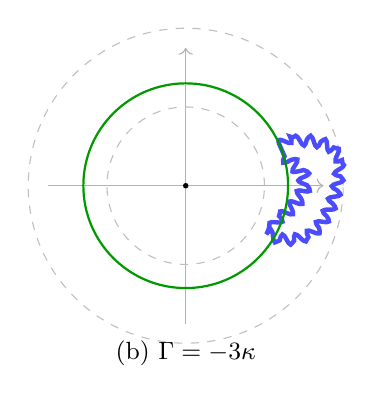
\begin{tikzpicture}[scale=0.5]
        \panel{2.6}{green!60!black}{}
        \node[below] at (0,-3.7) {\small (b) $\Gamma=-3\kappa$};
        \end{tikzpicture}
    }; &
    \node{
        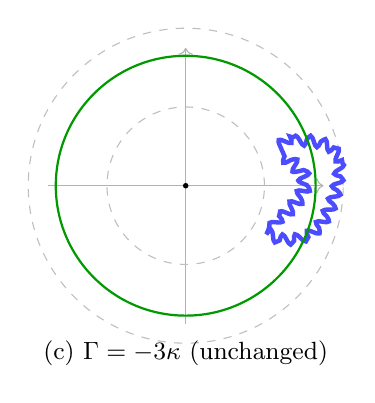
\begin{tikzpicture}[scale=0.5]
        \panel{3.3}{green!60!black}{}
        \node[below] at (0,-3.7) {\small (c) $\Gamma=-3\kappa$ (unchanged)};
        \end{tikzpicture}
    }; &
    \node{
        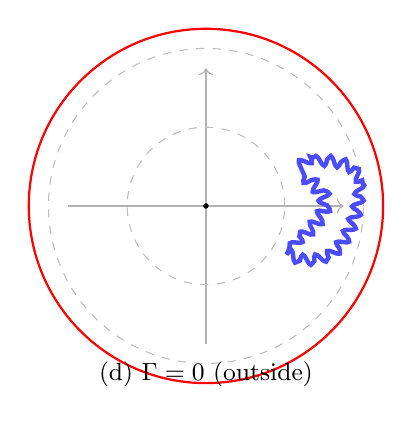
\begin{tikzpicture}[scale=0.5]
        \panel{4.5}{red}{}
        \node[below] at (0,-3.7) {\small (d) $\Gamma=0$ (outside)};
        \end{tikzpicture}
    };\\
};

\caption{Four-panel cartoon showing circulation around a trefoil’s central axis at different loop radii but fixed viewing geometry.
Panel (a): very small loop, no linking, $\Gamma=0$.
Panel (b): loop inside torus annulus, net linking number $q=3$, $\Gamma=-3\kappa$.
Panel (c): slightly larger loop still inside annulus: circulation unchanged (topological invariant).
Panel (d): very large loop outside annulus: net linking cancels, $\Gamma\approx 0$.}
\label{fig:fourpanel_circulation}


\end{tikzpicture}
\end{figure}